\section{Approach}
\label{sec:approach}

%\begin{figure*}[th!]
%	\centering
%	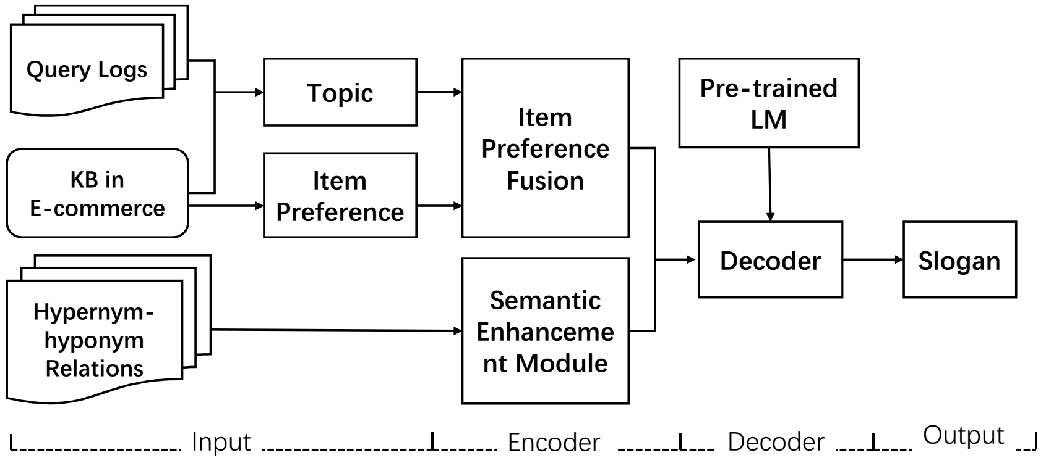
\includegraphics[width=1.6\columnwidth]{figures/flow}
%	\caption{Overall framework.}
%	\label{fig:flow}
%\end{figure*}

To generate informative and attractive slogans,
%In this section, 
we first review our basic convolutional 
sequence to sequence framework~\cite{gehring2017convolutional}. 
Then we present a novel model SSG 
which includes i) an item preference fusion module to reveal potential user interests; 
ii) a semantics-enhanced module for better deep semantic representations and selling point exploration by incorporating external knowledge.
Next, we describe these components.

%We first propose item preference fusion module to reveal potential user interests, then propose a semantics-enhanced module which incorporates \emph{is-a} knowledge for better contextualized representations and selling point exploration, and eventually generate informative and attractive slogans.

%which enriches the deep semantic representations with external knowledge and facilitate slogan generation in e-commerce.
%To generate generate informative and attractive slogans,
%SSG includes i) an item preference fusion module which reveals the potential user interests, then propose a semantics-enhanced module which incorporates \emph{is-a} knowledge for better contextualized representations and selling point exploration

% which includes   
%i) an item preference fusion mechanism to introduce 
%features of categorized items; 
%\emph{aspects} of coarse-grained concept which represents the shopping need of users;
%ii) semantics enhancement module incorporated hypernym-hyponym relations for better contextualized representation.
%SSG explores selling points and generates more informative and attractive slogans, bridging the semantic gap between latent user interests (refined shopping need) and 
%features of categorized items. 

%by explore features and selling points by incorporating  hypernym-hyponym relations;
%iii) language model integration at inference in order to benefit 
%from potentially limitless unsupervised text data and produce more fluent and reasonable slogans.



\subsection{An Encoder-Decoder Framework}
\label{sec:baseline}
In this section, we briefly introduce the basic framework, the convolutional sequence to sequence (CNN seq2seq\footnote{\url{https://github.com/facebookresearch/fairseq-py}}) model which is applied on slogan generation as a baseline model.
We later implement our proposed method based on this model.

Generally, the Seq2Seq framework consists of an encoder model to produce
a hidden representation of the source text, followed by a decoder model
to generate the target.
In our implementations, the model operated at the character level outperforms that at the word level. 
Thus we focus on the character-level tokens
processing in the following description.
Given the topic represent as an input sequence of characters
$\mathbf{ x } = (x_1, x_2, ..., x_n) $ and an product category $\mathbf{r}$
%embedded as $e_r$,
%as hints $r$, 
the objective of the system is to generate the textual slogan
$\mathbf{ y } = (y_1, y_2, ..., y_m) $,
a sequence of characters demonstrating the topic.


\paragraph{Encoder}
The encoder takes in the input text, and encodes it to a series of hidden 
representations.
Specially, the encoder embeds the character inputs 
$\textbf{x} = (x_{1},x_{2},...,x_{m})$ in distributional space
and obtains character embedding representations $\textbf{a} = (a_1, a_2, ..., a_m)$, 
where $a_i \in \mathbb{R}^f$ is a column in
an embedding matrix $A \in \mathbb{R}^{V\times f}$.
We embed the category $\mathbf{ r }$ to obtain the representation $r_e$.
Positional encoding is also applied in order to represent positional information,
which embeds the absolute position of inputs as $\textbf{b} = (b_1, b_2, ..., b_m)$,
where $b_i \in \mathbb{ R }^f$.
Both are combined to obtain input element representations $X = 
(X_1, X_2, ..., X_m)$, where $X_i = a_i+b_i+r_e$.
The encoder networks consists of $L$ convolutional layers.
Each layer is equipped with GLU \cite{DauphinFAG17} and residual connections \cite{HeZRS16},
ensuring that the sufficient and effective information is transmitted layer by layer.  
The output hidden states of $l$-th encoder layer is represented as 
$\textbf{z}^l = (z^l_1, z^l_2, ..., z^l_m)$.
Thus $z^l_i$ is computed as:
\begin{equation}
%\small
z _ { i } ^ { l } = ~ GLU \left( W ^ { l } \left[ z _ {i-k/2 } ^ { l - 1 } , \ldots , z _ { i+k/2 } ^ { l - 1 } \right] + b _ { w } ^ { l } \right)  + z _ { i } ^ { l - 1 }.
\end{equation}
The choice of $s$ and $t$ is up to kernel width $k$ and padding method.

\paragraph{Decoder}
The decoder is stacked with $L$ decoding layers as well.
Similar to the input representations $X$, 
$Y=(Y_1, Y_2, ..., Y_n)$ denote 
the distributional representations of output elements $y=(y_1, y_2, ..., y_n)$.
$\textbf{h}^l = (h^l_1, h^l_2, ..., h^l_n)$ denotes output states of the $l$-th decoder layer.
We compute the probability
distribution of generating the next elements $y_{i+1}$,
transforming $h_{i}^{L}$, the output state of the last decoder layer $L$ at $i$-th timesteps, via softmax:
%\begin{equation}
%%\small
%\begin{split}
%p \left( y _ { i + 1 } | y _ { 1 } , \ldots , y _ { i } , \mathbf { x } \right) = 
%& \operatorname { softmax } \left( W _ { o } h _ { i } ^ { L } + b _ { o } \right) \\ 
%&\in \mathbb { R } ^ { T }
%\end{split}
%\end{equation}
\begin{equation}
%\small
p \left( y _ { i + 1 } | y _ { 1 } , \ldots , y _ { i } , \mathbf { x } \right) = 
\operatorname { softmax } \left( W _ { o } h _ { i } ^ { L } + b _ { o } \right) \\ 
\in \mathbb { R } ^ { T }.
\end{equation}

In addition, a multi-step attention mechanism is introduced for each decoder layer.
To compute the attention, we combine the current decoder state
$h^l_{i}$ with an embedding of previously generated target element $Y_{i}$
as follows:
\begin{equation}
%\small
d _ { i } ^ { l } = W _ { d } ^ { l } h _ { i } ^ { l } + b _ { d } ^ { l } + Y _ { i }.
\end{equation}
For $l$-th decoder layer, the attention $a^l_{ij}$ of state $i$ and input element $j$
is computed as a dop-product between the decoder state summary 
$d^l_i$ and each output $z^L_j$ of the last encoder layer as follows:
\begin{equation}\label{eq:a}
%\small
a _ { i j } ^ { l } = \frac { \exp \left( d _ { i } ^ { l } \cdot z _ { j } ^ { L } \right) } { \sum _ { t = 1 } ^ { m } \exp \left( d _ { i } ^ { l } \cdot z _ { t } ^ { L } \right) }.
\end{equation}

The conditional input to the current 
decoder layer is a weighted sum of both encoder states and input element representations.
\begin{equation}\label{eq:c}
%\small
c _ { i } ^ { l } = \sum _ { j = 1 } ^ { m } a _ { i j } ^ { l } \left( z _ { j } ^ { L } + X_j \right)
\end{equation}
%where $z_{j}^{u}$ is the encoder output of last layer $u$.  
where the superscript $L$ indicates the last layer of encoder.  
Finally, $c _ { i } ^ { l }$ is added to $h_{i}^{l}$ as the input for the next decoder layer.


\subsection{Item Preference Fusion}
%\subsection{Item Preferences Construction}
\label{sec:preference}
A topic is a fluent and short phrase which is usually coarse-grained and associated with a set of items across multiple categories.
To refine the shopping need represented by the topic 
as potential user interests,
we use one affiliated product category $\mathbf{r}$ to introduce \emph{item preference}.
An item preference is represented as a subset of related items sampled from $\mathbf{ r }$.
Specifically, the item preference $p$ associated with topic $x$,
consists of a set of items 
$\{s_1, s_2, ..., s_u\}$. 
%	Different item preferences of a specific topic are expected to imply different focuses or selling-points according to their item members. 
$s_i$ is represented as a sequence tokens of its title.
Then, $p$ is the text sequence, concatenating $s_1, s_2, ..., s_u$. 
%One of the limitation of the baseline encoder-decoder framework
%is that it often drifts to irrelevant contents.
%The basic topic information is still far from enough
%for generating an accurate and informative slogan.
%Therefore one of the limitation of the baseline
%encoder-decoder framework is that
%it often gives general slogans and sometimes even irrelevant to the topics since the issue of inadequate contextual information.
%In addition, topics are usually coarse-grained and consists of items 
%across many secondary categories.
%in order to generate more accurate and attractive slogans,
%it is necessary to consider the item preferences of topics,
%enriching the input information as well as 
%highlighting the selling-points accordingly.
%Each category is associated with a number of items.
%Given a topic $w$, we first sample at most 10 popular secondary categories of $w$, then we sample a small set of items from each to formulate the item preferences
%$P$ for $w$.
%Thus $w$ provided with $p$, where $p \in P$, is assumed to 
%imply a focus or potential preference for users.
%$p$ consists of a set of items $\{s_1, s_2, ..., s_u\}$.
%$s_i$ is represented as the character sequence of the item title.
Based on the topic $x$ and its item preference $p$, we want to generate 
a slogan $y$.
We propose three fusion methods to combine $x$ with $p$ in the encoder networks as follows.

\begin{figure*}[th!]
	\centering
	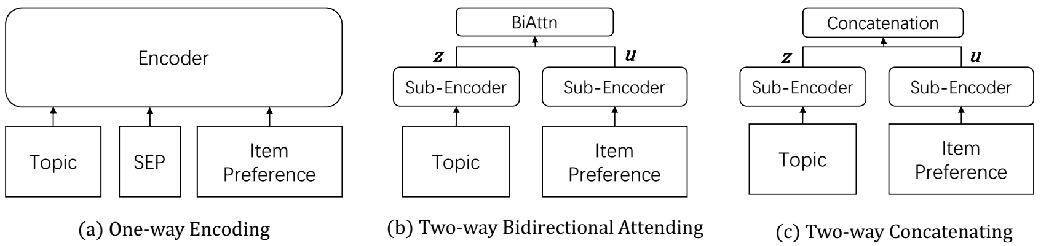
\includegraphics[width=1.8\columnwidth]{figures/enc}
	\caption{Three combinations of topic and item preference in the encoder of Seq2Seq model.}
	\label{fig:enc}
\end{figure*}


\paragraph{One-way Encoding}
We treat topic $x$ and its item preference $p$ homogeneously.
Thus, we concatenate $x$ with $p$ using a special token \emph{SEP} as the separator. Then we use the concatenated sequence as input to generate the 
slogan.
We demonstrate this fusion strategy in \figref{fig:enc} (a).
%\begin{figure}[th!]
%	\centering
%	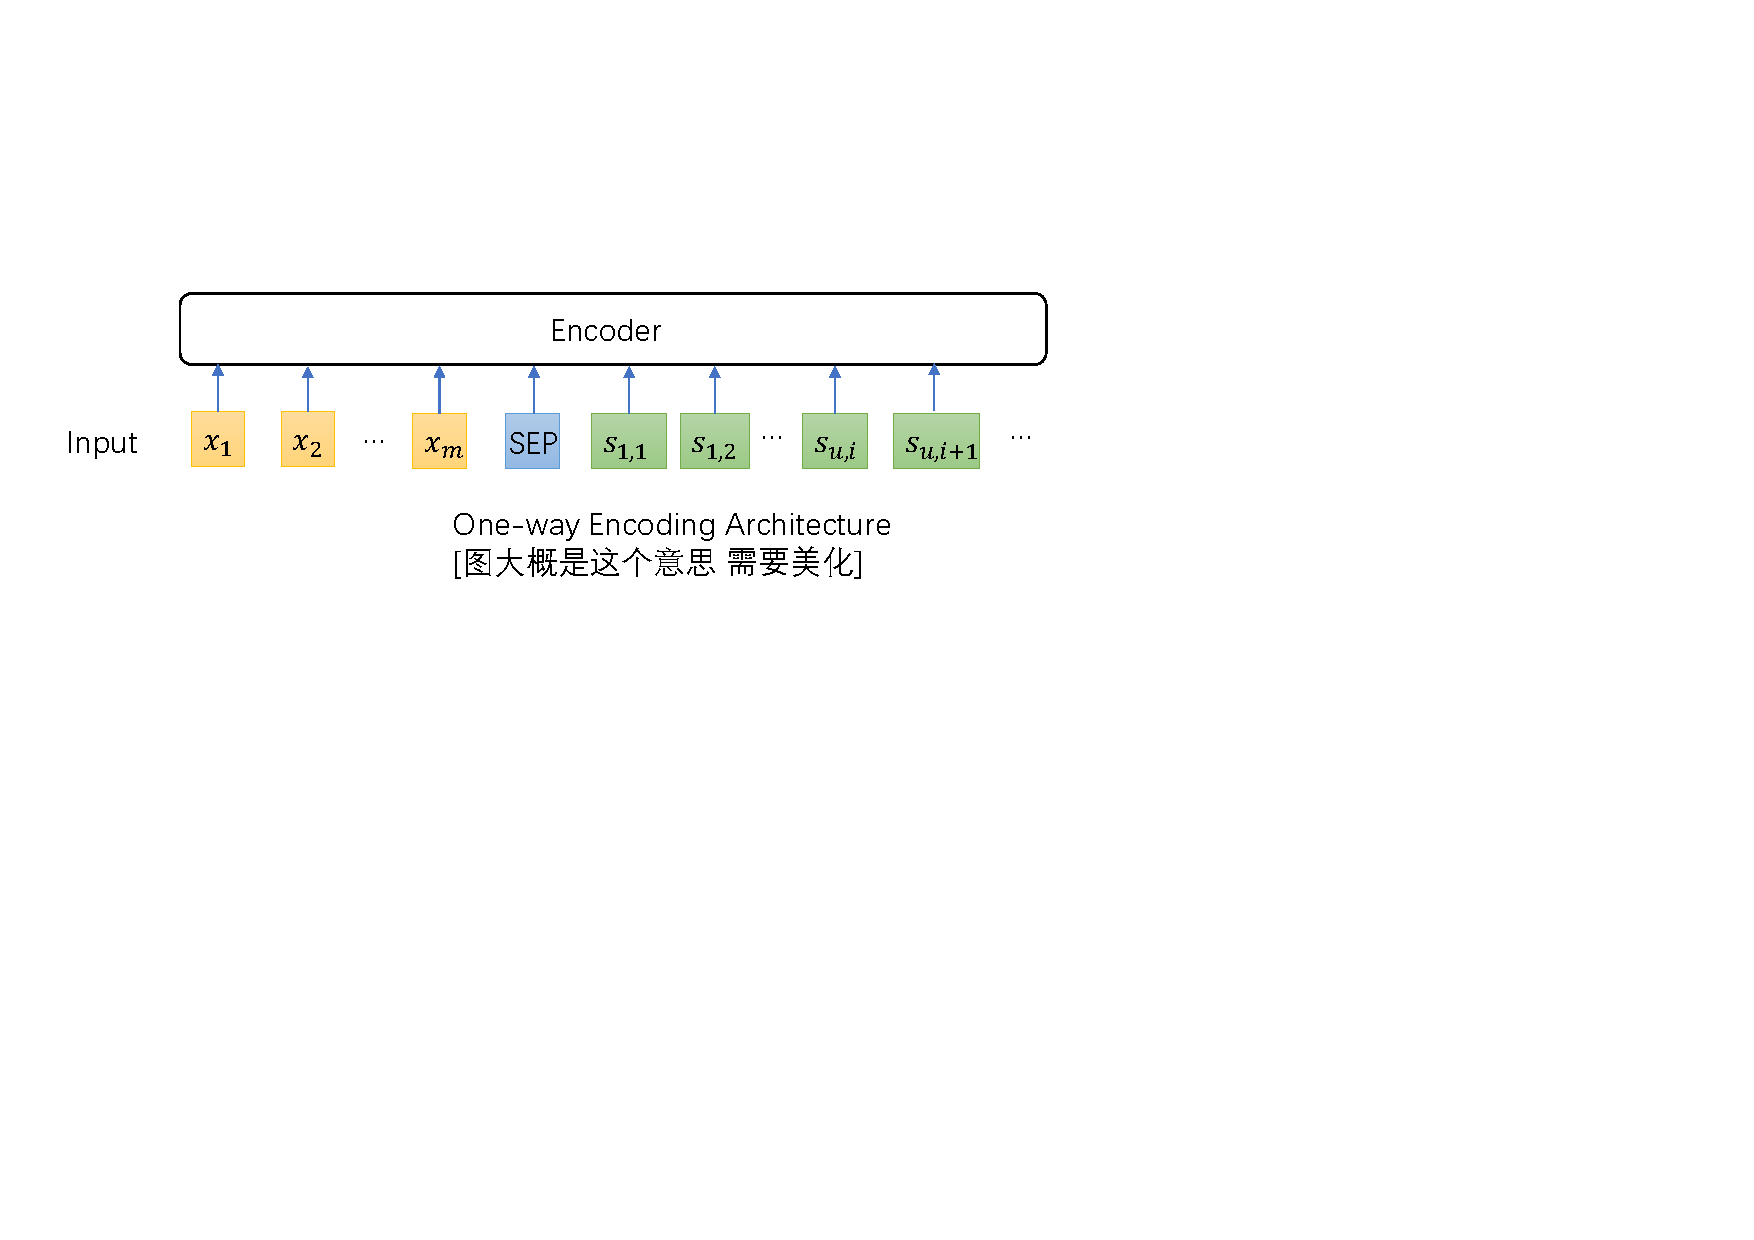
\includegraphics[width=0.95\columnwidth]{figures/oneway0}
%	\caption{xx.}
%	\label{fig:oneway}
%\end{figure}


\paragraph{Two-way Bidirectional Attending}
In fact, topic $x$ and its item preference $p$ are two heterogeneous inputs. Thus, we make the encoder consists of two sub-encoders to 
encode $x$ and $p$ separately.
%It is more reasonable to treat them differently.
We propose two-way bidirectional attending method as 
a alternative fusion method.
As shown in \figref{fig:enc} (b), after obtaining the encoded representation of $x$ as $\textbf{z}$ and that of $p$ as $\textbf{u}$, we combine the two kinds of representations using BiDAF ~\cite{seo2016bidirectional}.
%\begin{figure}[th!]
%	\centering
%	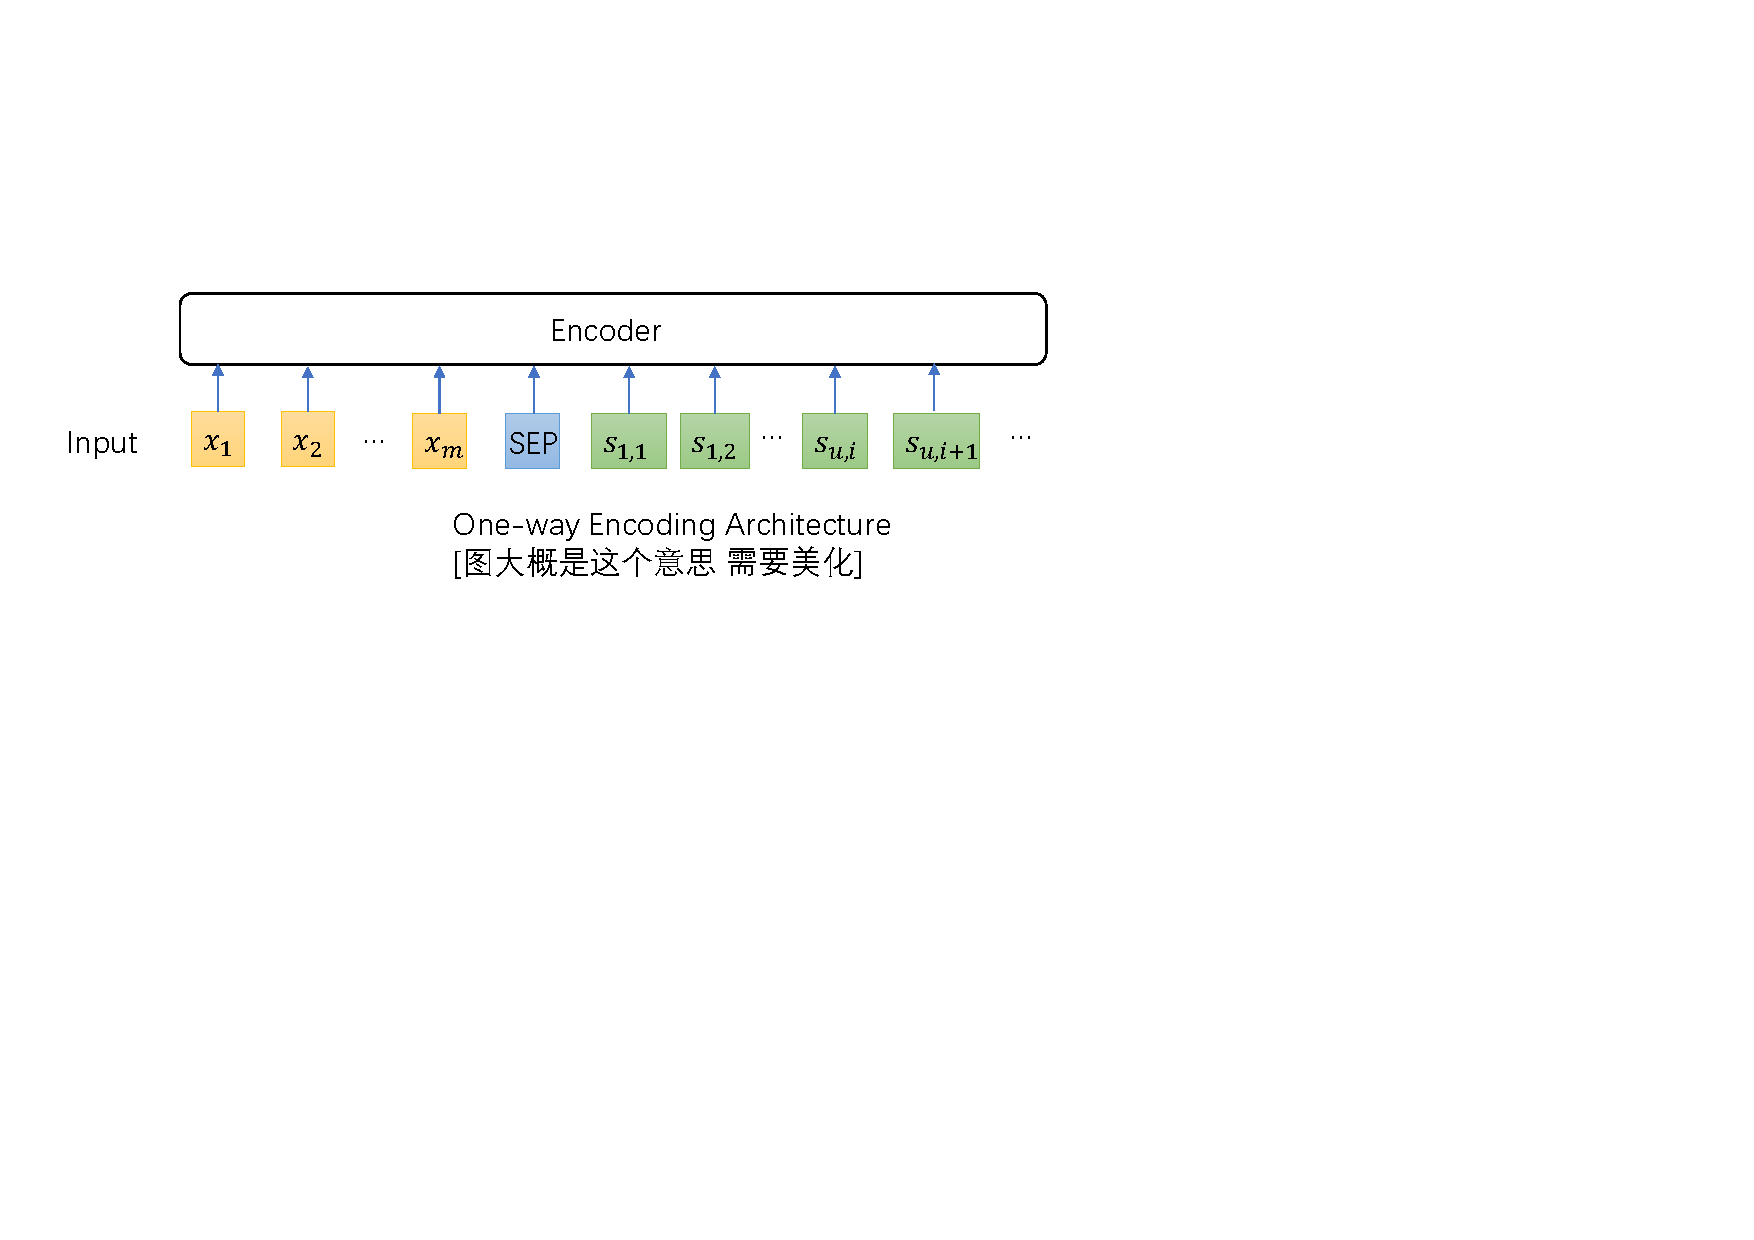
\includegraphics[width=0.95\columnwidth]{figures/oneway0}
%	\caption{xx.}
%	\label{fig:twoway_bi}
%\end{figure}

\paragraph{Two-way Concatenating}
Two-way concatenating also treats topic $x$ and item preference $p$ heterogeneously.
As shown in \figref{fig:enc} (c),
two-way concatenating method simply concatenate $z$ and $u$, the deep contextualized representations from two heterogeneous sub-encoders, as the output states of the encoder networks.
We show that this strategy outperforms previous two in \secref{sec:experiments}.

%\begin{figure}[th!]
%	\centering
%	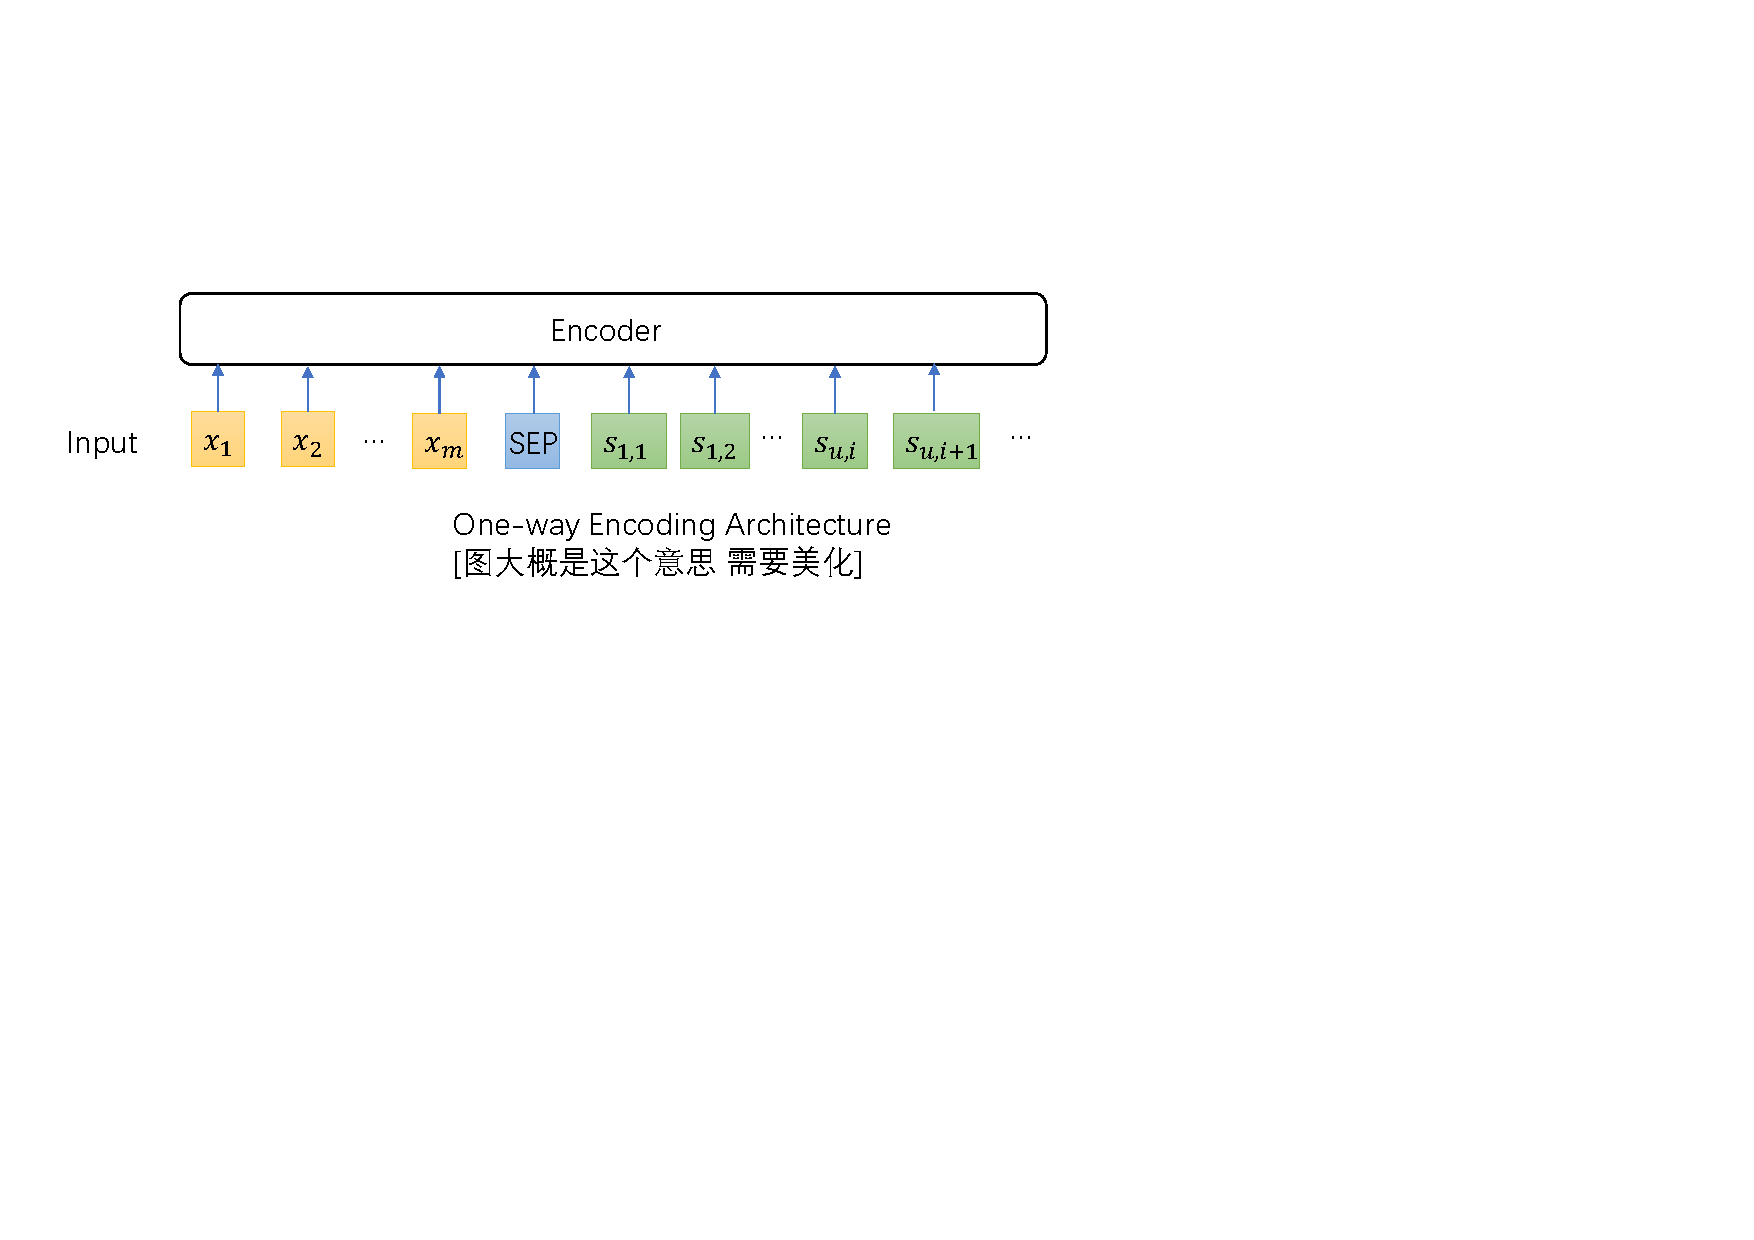
\includegraphics[width=0.95\columnwidth]{figures/oneway0}
%	\caption{xx.}
%	\label{fig:twoway_cat}
%\end{figure}

%  length of encoder output: L1+L2+1 / L2 / L1+L2


%\figref{fig:cate}
%\begin{figure}[th!]
%	\centering
%	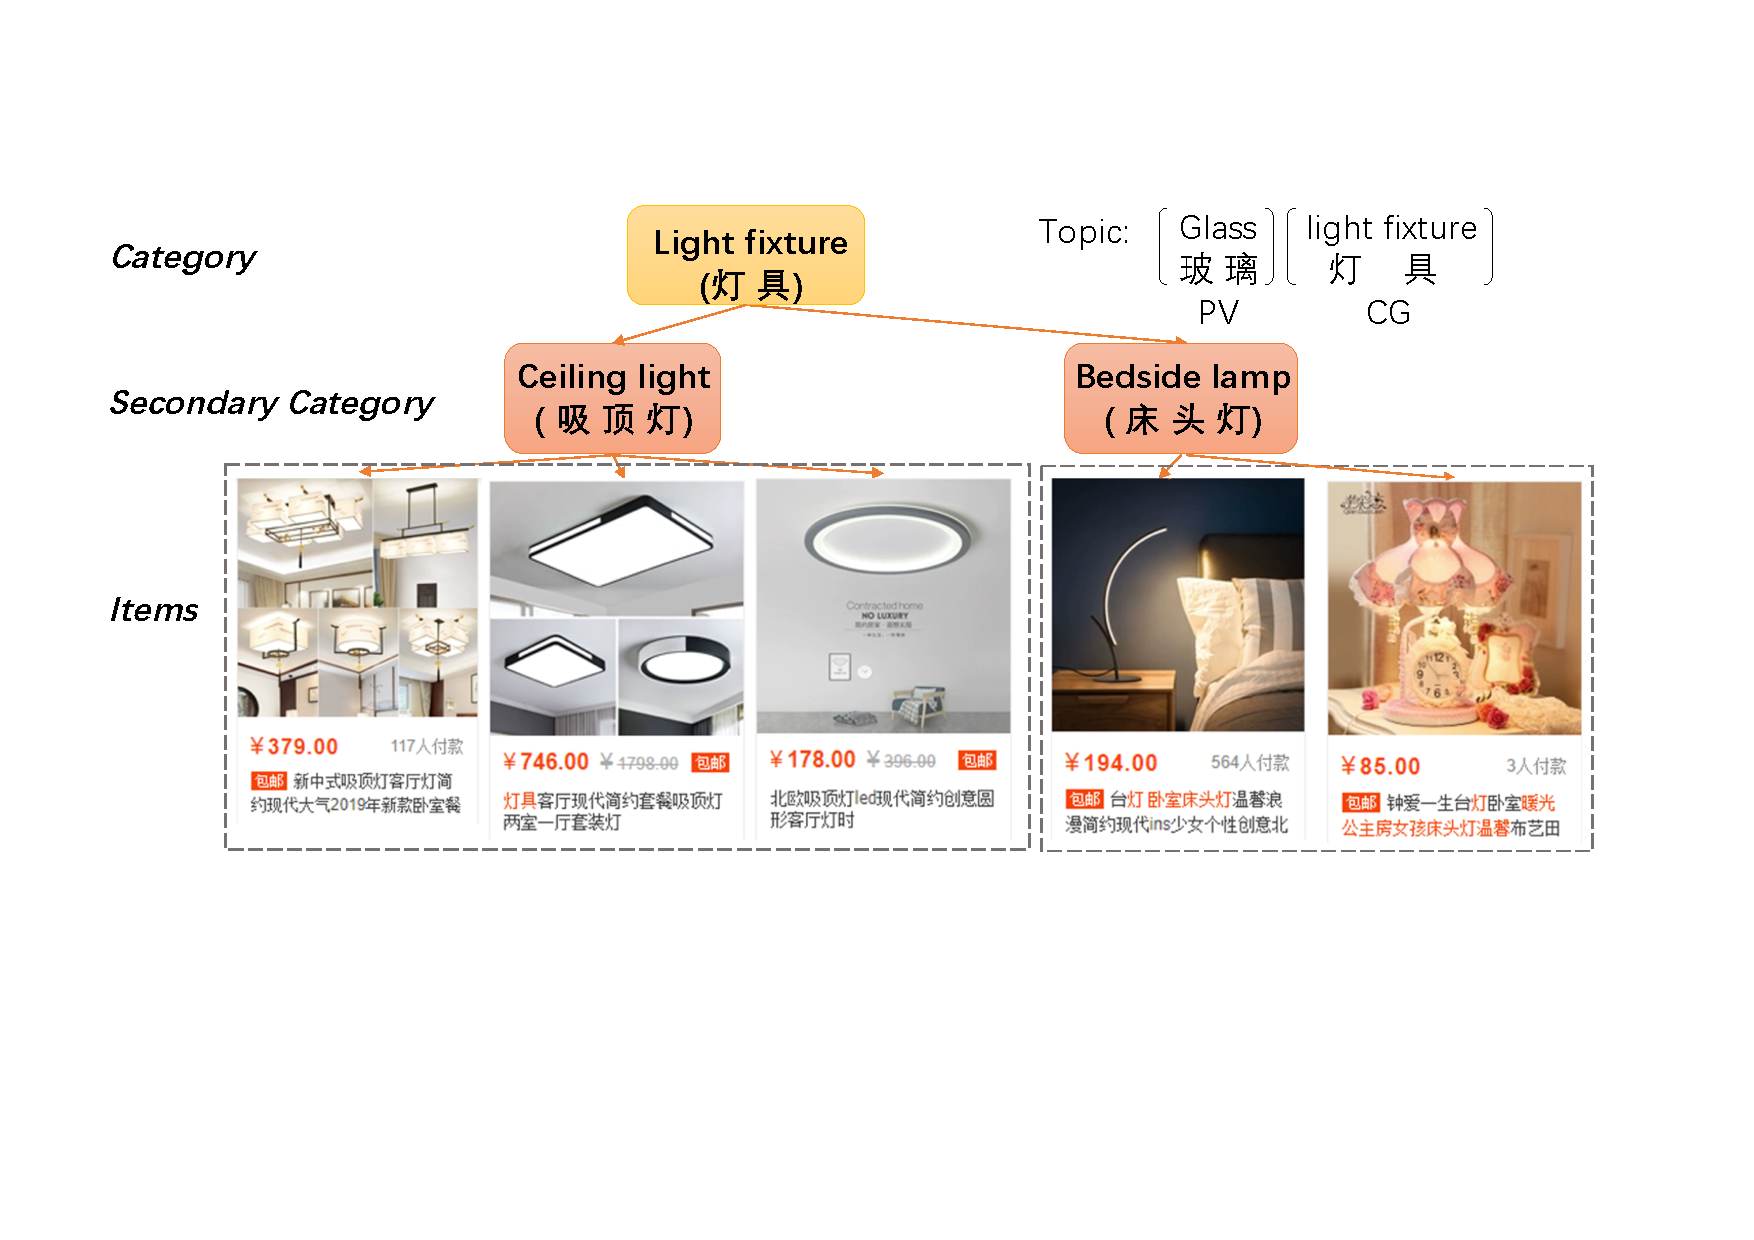
\includegraphics[width=0.95\columnwidth]{figures/cate8}
%	\caption{An example of category structure in E-commerce.}
%	\label{fig:cate}
%\end{figure}

\subsection{Semantics Enhancement}
\label{sec:semantics}
%Item preference consists of a set of items.
% intuition
Emperical results in \secref{sec:experiments} show that two-way concatenating is relatively effective for heterogeneous inputs combination.
%However, such concatenation of heterogeneous hidden states
Backed by two-way concatenating fusion, 
we propose a novel semantics enhancement module 
which effectively incorporates the semantic relations
between heterogeneous inputs,
to enhance the neural model
with enriched deep contextualized representations.
More specifically, 
$\textbf{z}=(z_1, z_2, ..., z_{L1})$ is the encoded representation of topic $x$,
where $z_i \in \mathbb{R}^{f}$.
$\textbf{u}=(u_1, u_2, ..., u_{L2})$ denotes the encoded representation of item preference $p$ of $x$, where $u_j \in \mathbb{ R }^{g}$.
Note that, we can use different dimensions for $z_i$ and $u_j$ ($f$ and $g$) here, 
since we treat $x$ and $p$ heterogeneously and encode them separately.
Then we later transform $z_i$ and $u_j$ into same dimension via linear layers in order to adapt to the two-way concatenating fusion method.
Next, we introduce hypernym-hyponym relations for the semantics enhancement module, which are collected from taxonomy $\mathcal{T}$, an essential component of  e-commerce knowledge graph
%~\footnote{We will release the hypernym-hyponym relations used in our experiments at https://202.120.38.146/slogan/},
.
We first identify the \emph{is-a} relations between topic $x$ and item preference $p$ 
(in \secref{sec:identification}),
then propose a \emph{is-a} knowledge-aware module for better contextualized representations
(in \secref{sec:combination}).
We present the semantics enhancement module
in \figref{fig:enhancement}

\subsubsection{Relation Identification}
\label{sec:identification}
To tighten the semantic connections between $x$ and $p$,
and further enhance the deep contextualized representations,
we conduct the identification as retrieving 
\emph{is-a} knowledge from $x$ for $p$.

Specifically, we first process $x$ and $p$ into entity sequences, represented as 
$(v_1, v_2, ..., v_X)$ and $(w_1, w_2, ..., w_P)$, where $v$ and $w$
are entities in $\mathcal{T}$,  in order to identify semantic relations in ease.
%We then identify the \emph{is-a} relations between them.
%More specially, 
For each entity $w$ extracted from $p$, 
we identify the \emph{is-a} relations 
between $w$ and $v$ by traversing every $v$ in $x$.
Thus, $w$ is related to $v$ in one of the following three cases:
 i) $w$ is a \emph{hypernym} of $v$, referred as \emph{hyper};
 ii) $w$ is a \emph{hyponym} of $v$, referred as \emph{hypo};
 and iii) $w$ is neither a hypernym nor a hyponym of $v$, referred as \emph{none}.
We suppose that entity $w=(p_s, p_{s+1}, ..., p_{t})$ is identified as \emph{rel} relation with 
entity $v = (x_o, x_{o+1}, ..., x_{q})$,
where $(x_1, x_2, ..., x_{L1})$ and $(p_1, p_2, ..., p_{L2})$ are
character-level sequences of $x$ and $p$.
For a entity such as $v$, we consider its hidden state at last position $z_q$
as a summary state for the $v$.
Thus, we associate the character at each position of $w$ in $p$, from $s$ to $t$,  to 
the character at last position $q$ of $v$ in $x$ with relation \emph{rel}
$\in \{hyper, hypo, none\}$.
For example, if $(w, hyper, v)$ is an identified \emph{hyper} triple 
(i.e. $w$ is a hypernym of $v$), 
where $w=(p_s, p_{s+1}, ..., p_{t})$ is the \emph{head} entity from $p$, 
$v = (x_o, x_{o+1}, ..., x_{q})$ is the \emph{tail} entity from $x$,
we obtain a bunch of character triples such as $(p_s, hyper, x_q)$, 
$(p_{s+1}, hyper, x_q)$, ..., $(p_{t-1}, hyper, x_q)$, $(p_{t}, hyper, x_q)$.
%As shown in \figref{fig:enhancement},
%``吸顶灯" (ceiling light) is a hyponym of ``灯具" (light fixture).
%Since ``具" is at the last position in ``灯具", we associate each character
%of ``吸顶灯" to ``具", we harvest triples
%as (吸, \emph{hypo}, 具), (顶, \emph{hypo}, 具) and (灯, \emph{hypo}, 具).
Note that, we ensure each character $p_j \in p$ is associated to one 
character $x_i \in x$ with a certain $rel$. 
If $p_j$ is not identified as a character in any entities, 
it is associated to a fake character $x_{\emptyset}$ with relation \emph{none}.

%A $w$ is possible to be identified with multiple $v$s
%Note that, $w$ can be identified with multiple $v$s 

%the semantic relations as linear transformation matrices.
%We remark the 

%We suppose that $(x_1, x_2, ..., x_{L1})$ and $(p_1, p_2, ..., p_{L2})$ are
%character-level sequences of $x$ and $p$.
%$w=(p_s, p_{s+1}, ..., p_{t})$ denotes that 
%Similarly, $v = (x_o, x_{o+1}, ..., x_{q})$.


\subsubsection{Semantics Combination}
\label{sec:combination}
%Next, we conduct the semantics combination
%to incorporates the identified relations
%and enhance the semantics representation
%of the encoder backed by two-way concatenating fusion framework.
After relation identification, 
each character $p_j \in p$ has been associated to 
a character $x_i \in x$ with a specific relation \emph{rel},
where \emph{rel} $\in \{ hyper, hypo, none\}$.
For the character $p_j$ associated to $x_i$ with \emph{rel} relation,
we attempt to enhance the semantic representation $u_j$ 
based on $z_i$ according to \emph{rel}.
We introduce a linear transformation matrix $W^{rel} \in \mathbb{ R }^{(f+g) \times f}$ for semantic relation \emph{rel}
in order to combine  $u_j$ (the semantic representation of tail $x_i$) with 
$z_i$ (the representation of head $p_j$) accordingly.
%in order to transform $z_i$ (the representation of tail $x_i$)
% into semantic space same as $u_j$ (the representation of head $p_j$).
% and the tail $x_i$ into same semantic space. 
We concatenate $u_j$ and $z_i$ as $[u_j; z_i] \in \mathbb{ R }^{2f}$ followed by 
the semantics transformation 
to form the semantic-enhanced representation
as $\tilde{u}_j = W^{rel}[u_j ; z_j] \in \mathbb{ R }^{f}$.
Then we use $\tilde{\textbf{u}} = (\tilde{u}_1, \tilde{u}_2, ..., \tilde{u}_{L2})$
as the sub-encoder output representations of item preference $p$.
Note that, $z_{\emptyset}$, the representation of fake token $x_{\emptyset}$ is set to be a vector full of zeros.
Backed by two-way concatenating fusion mechanism, 
we use a simple concatenation of hidden states $[\textbf{z}; \tilde{\textbf{u}}] \in \mathbb{ R }^{f\times (L1+L2)}$ to get the final combined representation.





\begin{figure}[th!]
	\centering
	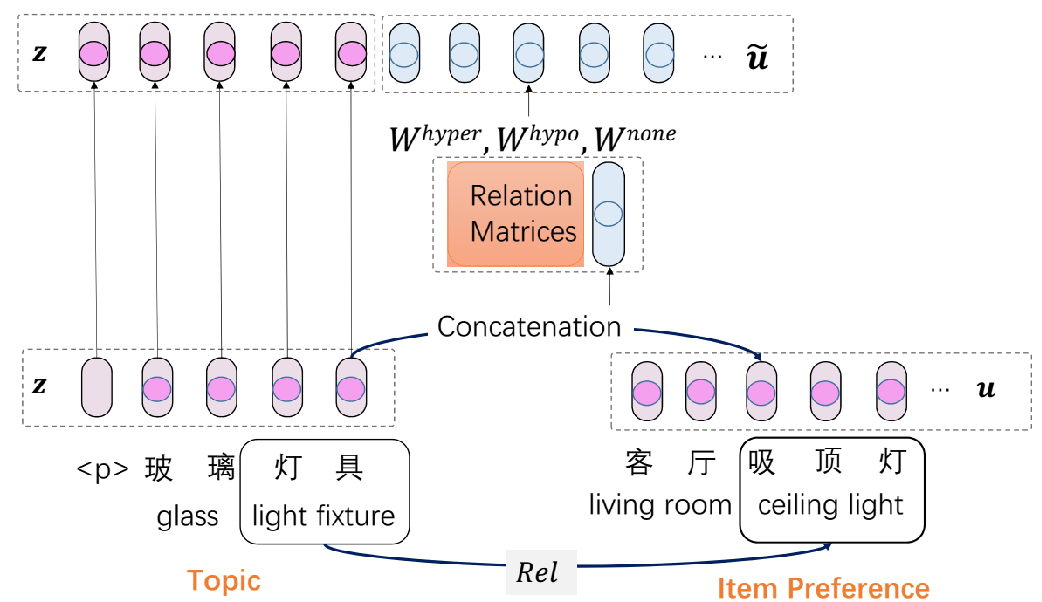
\includegraphics[width=1.0\columnwidth]{figures/enhancement}
	\caption{The semantics enhancement module in details.}
	\label{fig:enhancement}
\end{figure}


%We introduce a linear transformation matrix $W^{rel} \in \mathbb{ R }^{g \times f}$ for semantic relation \emph{rel}
%in order to transform $z_i$ (the representation of tail $x_i$)
%into semantic space same as $u_j$ (the representation of head $p_j$).
%% and the tail $x_i$ into same semantic space. 
%We concatenate $u_j$ and $W^{rel}z_i$ followed by a projection 
%to form the semantic-enhanced representation
%as $\tilde{u}_j = W^{proj}[u_j ; W^{rel}z_j] \in \mathbb{ R }^{f}$,
%where $W^{proj} \in \mathbb{ R } ^{f \times 2f }$.
%Then we use $\tilde{\textbf{u}} = (\tilde{u}_1, \tilde{u}_2, ..., \tilde{u}_{L2})$
%as the sub-encoder output representations of item preference $p$.
%Note that, $z_{\emptyset}$, the representation of fake token $x_{\emptyset}$ is set to be a vector full of zeros.
%Backed by two-way concatenating fusion, 
%we use a simple concatenation $[]$ to get the final combined representation.
%


We assume that the exploration of semantic relations further tighten the connections between 
the heterogeneous inputs.
Moreover, the semantics enhancement module is aware of \emph{is-a} relations,
it learns to use \emph{is-a} knowledge to increase the semantic capacity of the model 
for proficient contextualized representations.
This effect is demonstrated empirically in \secref{sec:experiments} where
semantics-enhanced models outperforms other baselines on various evaluation metrics.


\cut{
\subsection{Pretrained Language Model Integration}
\label{sec:shallow_fusion}
% potential limitless, reasonable, fluent
% other domain, robustness
The sequence-to-sequence framework trains directly maximizes the probability
of observing desired outputs conditioned on the inputs.
This discriminative mode allows Seq2Seq model to focus on the most informative 
features.
However, it also increases the risk of overfitting to those few distinguishing
characteristics.
Thus, the Seq2Seq model tends to yield very sharp predictions 
and only a few hypotheses need to be considered to find the most 
reasonable targets.
Such high confidence mainly manifests as low diversity of targets obtained 
using beam search.
Another limitation is that native Seq2Seq framework is trained to generate 
complete sequences without a language model, 
its decoder learns an implicit language model from the training corpus.
Besides, labeled parallel corpus on specific task is usually low-resource.
Thus, the decoder tends to be underfittly trained and bias towards the training labels.

On the other hand, language models can be trained from abundantly available
unsupervised text corpora which can implicitly learn commonsense knowledge
across domains. 
To ameliorate the limitations of Seq2Seq, 
we integrate a state-of-the-art pre-trained language model (PLM), 
BERT~\cite{devlin2018bert} to Seq2Seq model at inference.
BERT has been achieved tremendous success on lots of NLP tasks
due to its pre-trained knowledge on limitedness unsupervised text corpus.
Since pretraining on a large corpus is quite cost, 
we use BERT-Base for Chinese~\cite{wolf2019transformers}
for PLM integration. 

We linearly combine the score of the
task specific Seq2Seq model with that of pretrained language model
to guide beam search, referred as \emph{shallow fusion} proposed by
Gulcehre et al.~\cite{gulcehre2015using}.
In our case, we conduct shallow fusion in order to improve slogan generation system
on low-resource human-crafted training pairs. 
More specially, 
at each time step $t$,
our proposed model SALE computes score of every
possible next word for each hypothesis all of hypotheses $\{y^{(i)}_{\le t-1}\}$
, where superscript $i$ stands for the index of hypothesis.
During inferencing, 
each score is the summation of the score of the hypothesis and
the score given by the SALE to the next word.
All these new hypotheses (a hypothesis from the previous timestep with 
a next word appended at the end) are then sorted according to their
respective scores, and the top $K$ ones are selected as candidates
$\{y^{(i)}_{\le t}\}$, where $i = \{1, 2, ..., K\}$.
We then rescore these hypotheses with the weighted sum of the scores
by SALE and PLM such as BERT~\cite{devlin2018bert}.
The score of the new word is computed by
%~\eqref{eq:shallow_fusion}
\begin{equation}
\label{eq:shallow_fusion}
\begin{split}
\log p \left( y _ { t } = k \right)  =
	&	\log p_{SALE} \left( y_t = k \right) \\ 
	& + \beta \log p_{LM} \left(y_t = k\right),
\end{split}
\end{equation}
where $\beta$ is hyper-parameter that needs to be tuned to maximize the 
performance on a development set.

%Shallow fusion effectively integrates PLM 
% in order to benefit 
%from potentially limitless unsupervised text data and improve
%the generalization and robustness of the model, 
%thus further produces more reasonable slogans.
%This refers to Pre-trained LM module in \figref{fig:flow}.
%
}

